\begin{pa} \label{PA:6.1}  Consider the functions given by $f(x) = 5-(x-1)^2$ and $g(x) = 4-x$.

\ba
	\item Use algebra to find the points where the graphs of $f$ and $g$ intersect.
	\item Sketch an accurate graph of $f$ and $g$ on the axes provided, labeling the curves by name and the intersection points with ordered pairs.
	\item Find and evaluate exactly an integral expression that represents the area between $y = f(x)$ and the $x$-axis on the interval between the intersection points of $f$ and $g$.
	\item Find and evaluate exactly an integral expression that represents the area between $y = g(x)$ and the $x$-axis on the interval between the intersection points of $f$ and $g$. 
	\item What is the exact area between $f$ and $g$ between their intersection points?  Why?
\ea

\begin{figure}[h]
\begin{center}
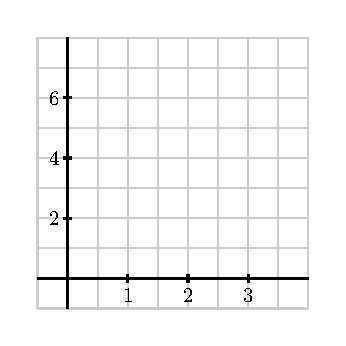
\includegraphics{figures/6_1_PA1.eps}
\caption{Axes for plotting $f$ and $g$ in Preview Activity~\ref{PA:6.1}} \label{F:6.1.Intro}
\end{center}
\end{figure}

\end{pa} 
\afterpa